 \documentclass[12pt]{article}
 \usepackage[
    left=1.25in,
    right=1.25in,
    top=1.5in,
    bottom=1.5in]{geometry}


\usepackage{apacite} 				% % literature-References: American Psycholog. Assoc.
\usepackage{natbib}					
\usepackage[hidelinks]{hyperref}
\hypersetup{
    colorlinks=true,
    linkcolor=blue,
    filecolor=magenta,      
    urlcolor=cyan,
    citecolor=blue,
    pdfborderstyle={/S/U/W 0}
}

\setcitestyle{round,aysep={}} 		% indexation in (round) parentheses, between the author year
\usepackage[utf8]{inputenc}
\usepackage[english]{babel}				% orthography
\usepackage[T1]{fontenc}
\usepackage{lmodern}				% font family
\usepackage{microtype}				% for micro typography (for a better typeface)
\usepackage{blindtext}
\usepackage{graphicx} 				% for including graphs (pdf,png - but do avoid jpg)
\graphicspath{{./Graphics/}}          % path to the pictures

\usepackage{url}					%  formatting URL (e.g. in the literature) 
  
\usepackage{tabularx} 				% for a better configuration of tables
\usepackage{longtable} 		
\usepackage{multicol}				
\usepackage{multirow}
\usepackage{booktabs}
\usepackage{tabularx}
\usepackage{xcolor}
\usepackage{varioref}
		
\usepackage[active]{srcltx}

\usepackage{listings}				% algorithm

\usepackage{mdwlist}				% lists

\usepackage{setspace} 				% setting of the lines (rows)
\newtheorem{mydef}{Merksatz}  		% if examples or mnemotechnic verses are used with continuous numeration 
\newtheorem{bsp}{Beispiel}

\usepackage{amsmath}				% for the writting of mathematical formula
\usepackage{calc}
\usepackage{footnote}				% footnotes
\usepackage{tablefootnote}			% footnotes in tables
\hyphenation{voll-st\"andigen}		% for defining word devisions globally

\setcounter{tocdepth}{2}			% levels which are displayed in the table of contents

 %__________________________________document____________________________


\begin{document}

% Title page shall not include header or foooter lines
\thispagestyle{empty}

% All elements shall be centered
\begin{center}

    \vspace*{-8mm}

    {\LARGE INSTITUTE OF FINANCE AND STATISTICS\\[1mm]}
    \large University of Bonn\\

    \vspace*{1cm}

    
\includegraphics[width=0.4\textwidth]{./Graphics/UNI_Bonn_Logo_Standard_RZ.eps}

    \vspace*{1cm}

    % Kind of Thesis => (Bachelor Thesis ,Diploma Thesis, Master Thesis, Seminar Thesis)
    {\Large \textbf{Seminar Paper in Academic Practice}}\\

    \vspace{1cm}

    % Title of the Thesis
    {\Large \textbf{Regression Trees}}\\
    \vspace{1.5cm}

    % Names of Authors
    {\LARGE Timothy Currie}\\[15mm]

    % Superverisor, contact data and submission date
    \parbox{120mm} {
        \begin{large}
            \begin{tabbing}
                Supervisor: \hspace{1.8cm} \= Dr. Elias Wolf\\[1.5mm]
                Semester:\> Summer Term 2024\\[1.5mm]
                Author:\>Timothy Jakob Currie\\[1.5mm] % alphabetic order (Surname)
                Matriculation-Nrs.:\> 50074426\\[1.5mm]
                %Address:\> Street Nr, Postal Code City\\[1.5mm]
                Email:\> s69tcurr@uni-bonn.de\\[1.5mm]
                Subject:\>Bachelor Economics\\[1.5mm]
                Submission:\> 25. August 2024\\[1.5mm]
            \end{tabbing}
        \end{large}
    }

\end{center}
\clearpage{\pagestyle{empty}\cleardoublepage}
 			% title
					% table of contents

% -----------------------------------
\pagenumbering{arabic}% Arabic page numbers (and reset to 1)



\begin{enumerate}
    \item Introduction, test
    \item Explaining Regression Trees
    \item Testing Regression Trees with Simulations
    \item Using Regression Trees housing Market Data
    \item Conclusions
\end{enumerate}


\section{Introduction}
aaaaaaaaaaaWhile linear regression, probably the most used method by empirical economist can be useful in many situations, it can be useful to look at where it fails, and different methods excel. Regression trees have been used in many situations, with many extension being developed greatly improving their usefulness. In this paper I will first give a short exposition on Regression Trees, their theory and extensions and applicatios and contrast them with linear regression. I will perform easily understandable simulations comparing Regression Trees and Linear Regression. Show how Regression Trees can be used on a Dataset on the housing Market.


 %_______________________________________________________ warum dieses Thema, motivation

Linear regression performs poorly on many kinds of data, particularly those with non-linear relationships and interaction effects. What might be a better approach for these situations? Regression Trees can be useful in many situations where linear regression falls short.

Regression trees are, a powerful machine learning technique for predictive modeling. Regression trees offer an alternative approach that can be useful in many situations. We will discuss their advantages over traditional linear regression methods, cover the basics of regression trees, compare them with linear regression, address the issue of overfitting, and introduce advanced ensemble methods like Bayesian Additive Regression Trees (BART).

[Figure: Can you guess where regression trees and where linear regression will perform better?]



 %_______________________________________________________ einordnung in die Literatur 

Hastie and Tibshirani's an Introduction to Statistical Learning serves as an eccelent introduction to Regression trees, while Tan and Roy (2019) can give a deeper dive on BART a powerful ensemble method. 

 %_______________________________________________________ was habe ich herausgefunden 

The simulations show how regression trees outperform linear regression on datasets with non lenear relationships. etc.

 %_______________________________________________________ inhaltsangabe, zusammenfassung 




 %_______________________________________________________ hauptteil _______________________________________________

\section{Regression Trees}

Regression Trees are a machine learning method, that splits the predictor space into subregions and makes predictios for each region. In doing so it doesn't make assumptions about linearity or non-interaction between different dimensions.

Regression trees split the predictor space into regions that minimize the residual sum of squares given by:

\begin{equation}
    \sum_{j=1}^{J} \sum_{i \in R_j} ( y_i- \hat{ y}_{R_j} )^2
\end{equation}


In each region, $\hat{y}$ simply takes on the mean of all observations in that region. Typically, we can't find the optimal regions. Instead, we use a greedy algorithm called Recursive binary splitting to find the optimal split to minimize prediction error at each stage. One will typicall continue the algorithm until some threshold is reached, such as each new split not leading to much improvment.

This model is clearly quite different from regular linear regression. Regression trees do not assume a linear relationship between predictors and the response. They also have more parameters that can be tweaked e.g. how many splits to perform. 

One other major benifit of Trees over Linear Regression is thet they capture interaction effects naturally. If for example being blong typically increases pay, but only for women, a Regression Tree will ofnet naturally split along gender and then, for women only, along haircolor. Whearas in a linear Regression the researcher would have to manually include terms for all interaction effects they want to study.

%%%%%%Problems
\subsection{Pruning}

Some of the main problems with Regression Trees are that they are easily prone to overfitting and that the greedy nature of the splitting algorithm doesn't necessarily create the best possible, or even close to the best possible carving up of the predictor space.




Cost complexity pruning (or pruning) is one popular way to improve Regression Trees. It counteracts overfitting by removing non-essential splits. We grow a large Tree and then use the following formula:

\begin{equation}
    \sum_{m=1}^{|T|} \sum_{i: x_i \in R_m} (y_i - \hat{y}_{R_j})^2 + \alpha|T|
\end{equation}

The process involves:

Selecting a parameter $\alpha$
For each $\alpha$, finding the subtree that minimizes the cost
Using cross-validation to select the best $\alpha$
Instead of evaluating a Model on the data we trained it on we evaluate it on a separate set.
Achieve a good tradeoff between bias and variance.
Large \( \alpha \) results in very small trees, small \( \alpha \) in larger trees.
The objective is to achieve a good tradeoff between bias and variance. A large $\alpha$ results in very small trees, while a small $\alpha$ results in larger trees.


\subsection{Ensemble Methods}
Even with pruning, trees often perform worse than other ML methods. Ensemble methods improve results by combining many regression trees. Each one contributes a small part to the overall prediction. These can be independent of previous trees (e.g., Random Forests) or grown on the residuals of the current fit (e.g., Bayesian Additive Regression Trees - BART).

BART models the response as a sum of many tree-based models plus noise:

\begin{equation}
    Y_i = \sum_{j=1}^{m} g(X_i; T_j, M_j) + \epsilon_i
\end{equation}

BART calculates the residuals of the current sum of Trees, then modifies one Tree to decrease the residuals. It then takes the average over all but the burn-in iterations. Unlike single trees, BART avoids overfitting by averaging the predictions of many trees and provides a probabilistic prediction, giving a measure of uncertainty.

 %_______________________________________________________ modellbeschreibung


 %_______________________________________________________ methodik


 %_______________________________________________________ theorie 


 %_______________________________________________________ simulationen 

\section{Simulations}

Simulations can serve as a testing ground for statistical methos, allowing for easyer repetability and eleminating many of the complications that arise when using datasets.

On two datasets 

We ran simulations 400 times with regression trees having 4 terminal nodes. We compared the Mean Squared Error (MSE) for both methods. The data was generated as: $Y = \beta_0 + \beta_1X + \epsilon$, where $\epsilon \sim N(0, \sigma^2)$.

\begin{figure}
    \centering
    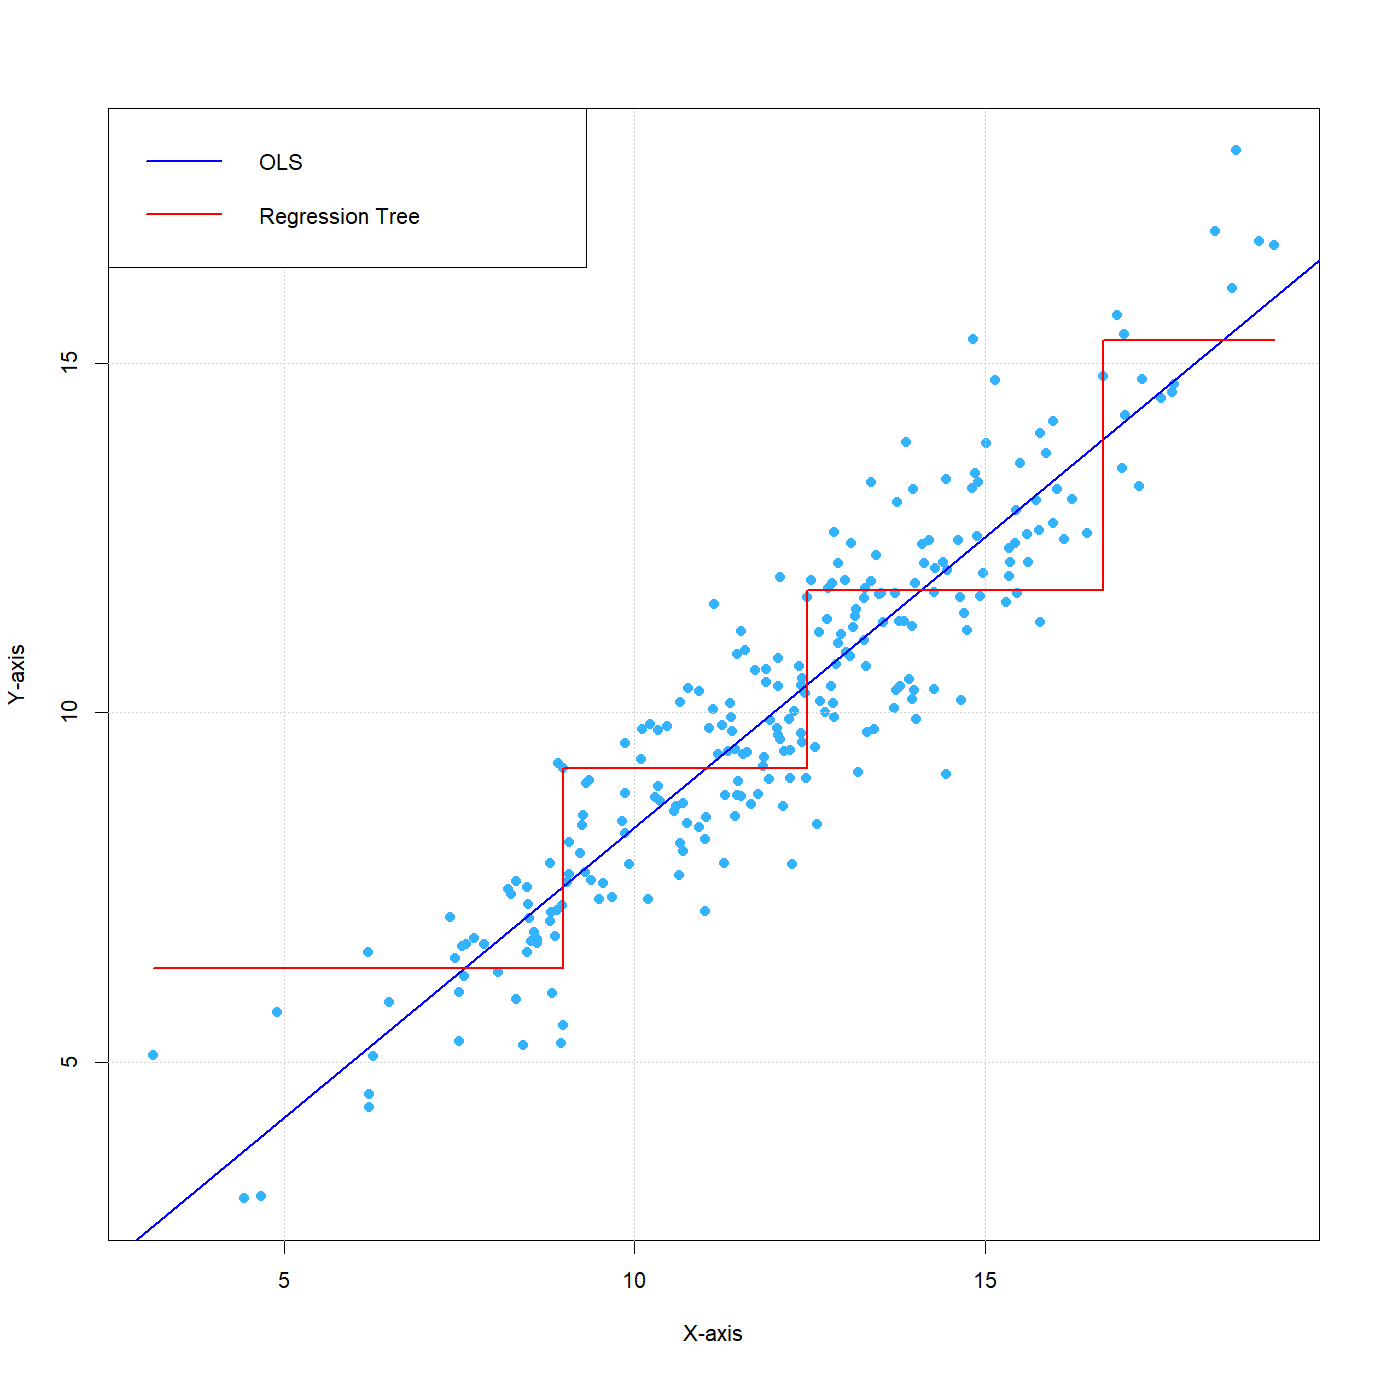
\includegraphics[scale=0.50]{OLS vs Tree.png}
    \caption{Linear Relation between Variables}
    \label{fig:sub1}  % Changed label to be unique
\end{figure}


Results:
\begin{itemize}
    \item MSE for OLS model: 0.9917 
    \item MSE for regression tree model: 1.4935 
\end{itemize}


\subsection{Non-linear Data}
We generated non-linear data using 4 normal distributions (NW and SE = red, NE and SW = blue). The results showed:


\begin{figure}
    \centering
    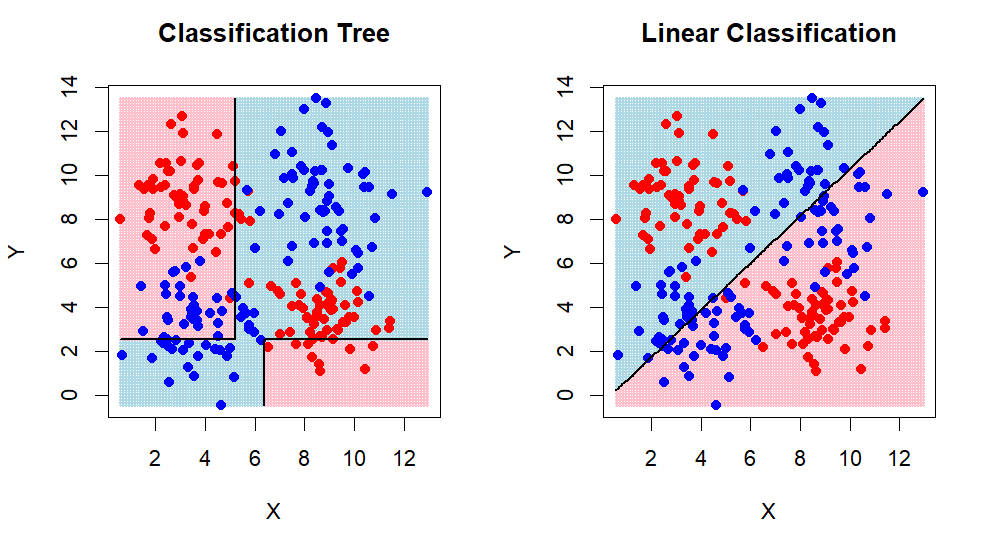
\includegraphics[scale=0.50]{NLD Pred.png}
    \caption{Data with Prediction}
    \label{fig:sub2}  % Changed label to be unique
\end{figure}


\begin{itemize}
    \item Classification Tree MSE: 0.3757
    \item Linear Classification MSE: 0.5103
\end{itemize}

Trees capture interaction effects better. For example, a large Y is only indicative of red if X is small.




Here you can see how the split that was made in the original tree was not the best possible split. It was greedy and couldn't look ahead.



\begin{figure}
    \centering
    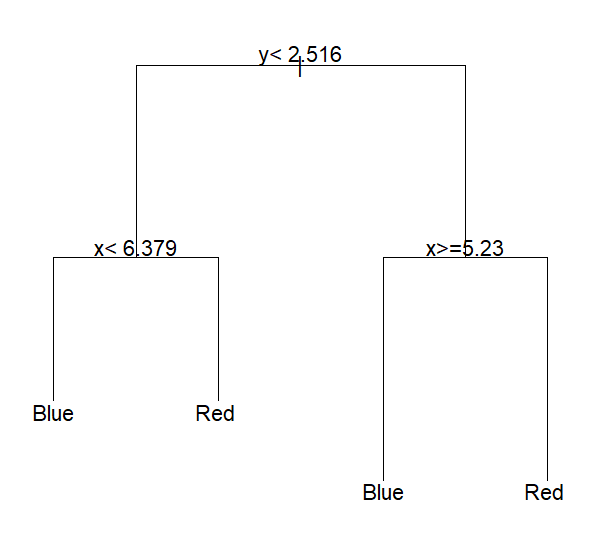
\includegraphics[scale=0.50]{Greedy Classification Tree.png}
    \caption{Greedy Classification Tree}
    \label{fig:sub3}  % Changed label to be unique
\end{figure}%


\subsection{Finding the Optimal Tree Size}
In our simulation:
\begin{itemize}
    \item Original Tree MSE on Test set = 198.2861 
    \item Pruned Tree MSE on Test set = 173.861 
\end{itemize}


The sweet spot balances variance and bias, minimizing overfitting. We use a training set to build the model and a test set to evaluate performance.


\begin{figure}
    \centering
    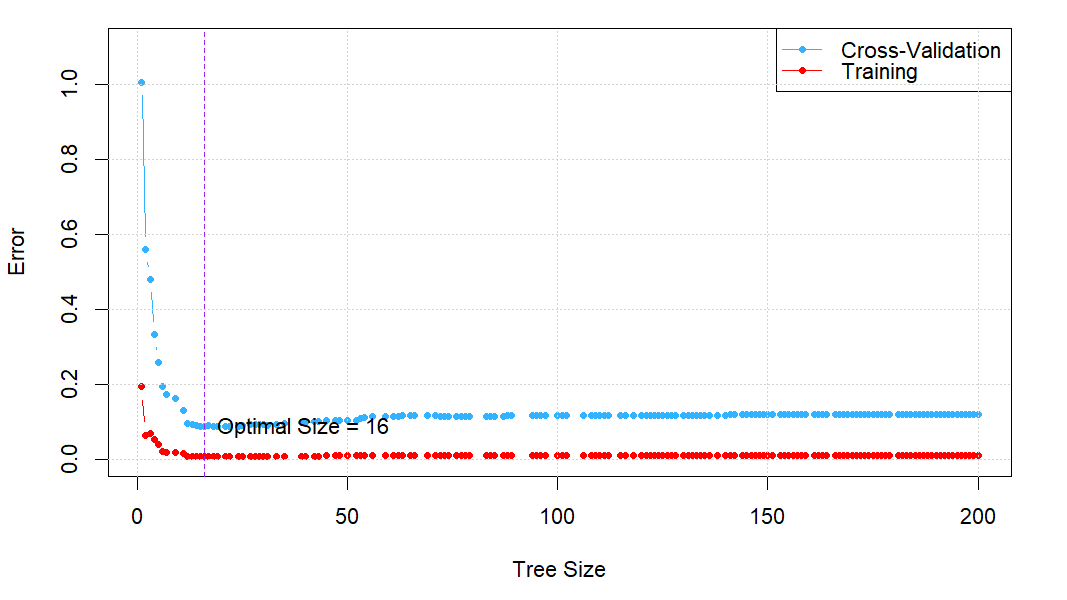
\includegraphics[scale=0.50]{Pruning.png}
    \caption{Training and Cross-Validation Error}
    \label{fig:sub4}  % Changed label to be unique
\end{figure}



 %_______________________________________________________ auf echte Daten 

\section{Applying Regression Trees To Housing Market Data}


and so on



 %_______________________________________________________ schlussbemerkungen __________________________________________



 \section{Conclusion}
Regression trees are powerful tools for handling non-linear and interactive effects, often outperforming linear regression in these scenarios. They are also very easy to interpret. However, trees require pruning to combat overfitting. Ensemble methods, by averaging independent trees or fitting trees on the residuals, can significantly improve results. BART, in particular, is a sophisticated method offering good results in many scenarios. While regression trees have their strengths, it's important to choose the right tool for each specific data analysis task.

 
 %_______________________________________________________ Ergebnisse kurz zusammenfassung

\subsection{Results and short summary}
and so on


 %_______________________________________________________ Offene Fragen

This is a very important area of research and clearly there are still many open questions.


 \section{References}
\begin{itemize}
    \item James, G., Witten, D., Hastie, T., Tibshirani, R. (2021). An Introduction to Statistical Learning with Applications in R (Second Edition). Springer.
    \item Tan, Y. V., Roy, J. (2019). Bayesian additive regression trees and the General BART model. Statistics in Medicine, Band/Volume 38(25), 5048-5069.
    \item Chipman, H. A., George, E. I., McCulloch, R. E. (2010). BART: Bayesian additive regression trees. The Annals of Applied Statistics, Band/Volume 4(1), 266-298.
    \item Townshend, R. Lecture 10 - Decision Trees and Ensemble Methods | Stanford CS229: Machine Learning (Autumn 2018). https://www.youtube.com/watch?v=wr9gUr-eWdA, accessed 21.05.24.
    \item All images were made using R. Also thanks to Claude and ChatGPT for making \LaTeX\ a lot nicer to use.
\end{itemize}


\end{document}